\chapter[Related Work]{Related Work}
\markboth{Chap. 2\ \ \enspace Background}{Chap 2. Background}

\regularsection
\headerregularsection

\updatemylof % to be used with "list of figure divider per chapter" (see PREAMBLE)

\begin{sloppypar} % to suppress overfull box


  At present, vision-based vehicle object detection is divided into traditional machine vision methods and complex deep learning methods. Traditional machine vision methods use the motion of a vehicle to separate it from a fixed background image. This method can be divided into three categories \cite{abdulrahim2016traffic}: the method of using background subtraction \cite{radhakrishnan2013video}, the method of using continuous video frame difference \cite{li2011vehicles}, and the method of using optical flow \cite{6746425}. Using the video frame difference method, the variance is calculated according to the pixel values of two or three consecutive video frames. Moreover, the moving foreground region is separated by the threshold \cite{li2011vehicles}. By using this method and suppressing noise, the stopping of the vehicle can also be detected \cite{park2007video}. When the background image in the video is fixed, the background information is used to establish the background model. Then, each frame image is compared with the background model, and the moving object can also be segmented. The method of using optical flow can detect the motion region in the video. The generated optical flow field represents each pixel’s direction of motion and pixel speed \cite{674625}. Vehicle detection methods using vehicle features, such as the Scale Invariant Feature Transform (SIFT) and Speeded Up Robust Features (SURF) methods, have been widely used. For example, 3D models have been used to complete vehicle detection and classification tasks \cite{BMVC.9.13}. Using the correlation curves of 3D ridges on the outer surface of the vehicle \cite{1570927}, the vehicles are divided into three categories: cars, SUVs, and minibuses.

  The use of deep convolutional networks (CNNs) has achieved amazing success in the field of vehicle object detection. CNNs have a strong ability to learn image features and can perform multiple related tasks, such as classification and bounding box regression \cite{zhao2019object}. The detection method can be generally divided into two categories. The two-stage method generates a candidate box of the object via various algorithms and then classifies the object by a convolutional neural network. The one-stage method does not generate a candidate box but directly converts the positioning problem of the object bounding box into a regression problem for processing. In the two-stage method, Region-CNN (R-CNN) \cite{6909475} uses selective region search \cite{uijlings2013selective} in the image. The image input to the convolutional network must be fixed-size, and the deeper structure of the network requires a long training time and consumes a large amount of storage memory. Drawing on the idea of spatial pyramid matching, SPP NET \cite{kaiming2014jian}  allows the network to input images of various sizes and to have fixed outputs. R-FCN, FPN, and Mask RCNN have improved the feature extraction methods, feature selection, and classification capabilities of convolutional networks in different ways. Among the one-stage methods, the most important are the Single Shot Multibox Detector (SSD) \cite{liu2016ssd} and You Only Look Once (YOLO) \cite{7780460} frameworks. The MutiBox \cite{6909673}, Region Proposal Network (RPN) and multi-scale representation methods are used in SSD, which uses a default set of anchor boxes with different aspect ratios to more accurately position the object. Unlike SSD, the YOLO \cite{7780460} network divides the image into a fixed number of grids. Each grid is responsible for predicting objects whose centre points are within the grid. YOLOv2 \cite{8100173} added the BN (Batch Normalization) layer, which makes the network normalize the input of each layer and accelerate the network convergence speed. YOLOv2 uses a multi-scale training method to randomly select a new image size for every ten batches. Our vehicle object detection uses the YOLOv3 \cite{redmon2018yolov3} network. Based on YOLOv2, YOLOv3 uses logistic regression for the object category. The category loss method is two-class cross-entropy loss, which can handle multiple label problems for the same object. Moreover, logistic regression is used to regress the box confidence to determine if the IOU of the a priori box and the actual box is greater than 0.5. If more than one priority box satisfies the condition, only the largest prior box of the IOU is taken. In the final object prediction, YOLOv3 uses three different scales to predict the object in the image.

The traditional machine vision method has a faster speed when detecting the vehicle but does not produce a good result when the image changes in brightness, there is periodic motion in the background, and where there are slow moving vehicles or complex scenes. Advanced CNN has achieved good results in object detection \cite{cai2016unified, hu2018sinet}; however, CNN is sensitive to scale changes in object detection. The one stage method uses grids to predict objects, and the grid’s spatial constraints make it impossible to have higher precision with the two-stage approach, especially for small objects. The two stage method uses region of interest pooling to segment candidate regions into blocks according to given parameters, and if the candidate region is smaller than the size of the given parameters, the candidate region is padded to the size of the given parameters. In this way, the characteristic structure of a small object is destroyed and its detection accuracy is low. The existing methods do not distinguish if large and small objects belong to the same category. The same method is used to deal with the same type of object, which will also lead to inaccurate detection. The use of image pyramids or multi-scale input images can solve the above problems, although the calculation requirements are large.


Detection of specific objects in images is difficult, due to the nature of objects in images that are often of different sizes, different orientations, and overlapping objects that causes occlusion of the object of interest to be detected \cite{ARINALDI201859}. These problems require a detection algorithm that has several properties, such as translation invariance(invariant to different locations of object of interest in the image), rotation invariance (invariant to the rotation of the object in the image), and scale invariance (invariant to the size of the objects in the image). A common approach is to use machine learning methods that learn a representation directly from the available data to train a model. Popular Methods use low level features such as SIFT \cite{lowe2004distinctive}, HOG \cite{dalal2005histograms}, and Haar \cite{viola2001rapid} combining them with a machine learning method to classify the objects. This approach is known as the "Feature +Classifier" approach.

\end{sloppypar}

%\begin{figure} % \begin{figure} will let LaTeX decide the best figure placement for you ; \begin{figure}[H] for forcing the figure placement here ; in the bottom, \begin{figure}[!b] ; top of the page, \begin{figure}[!t]
%    \centering
%    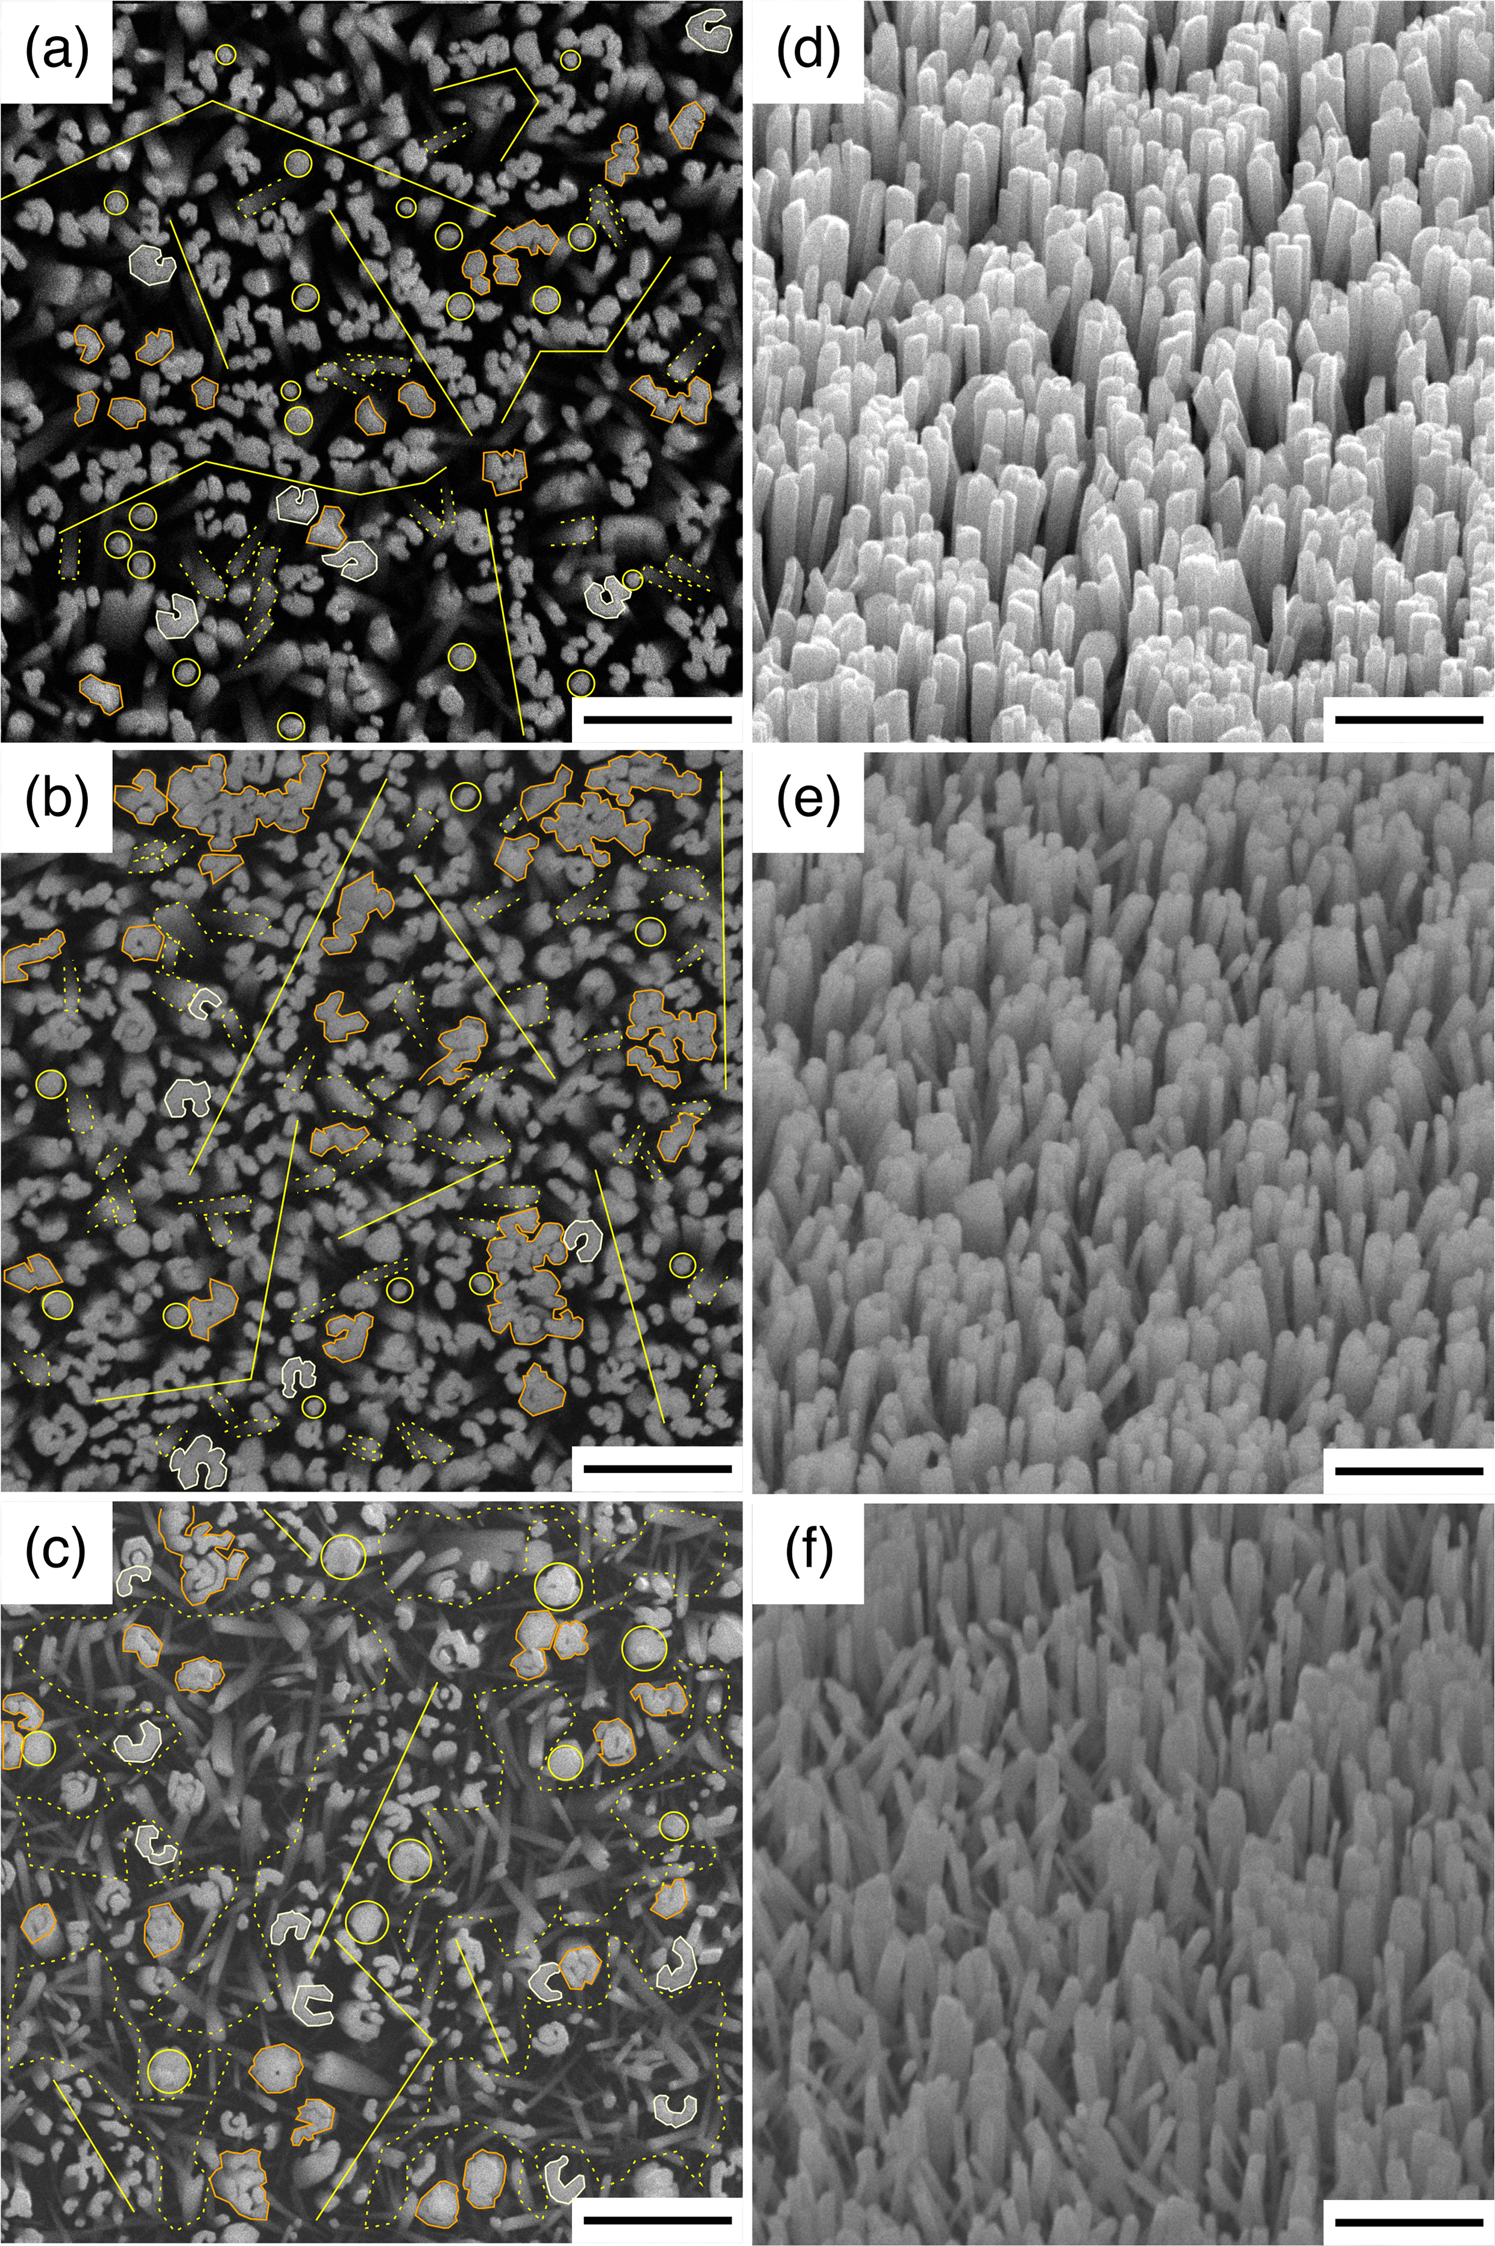
\includegraphics[width=0.95\textwidth]{figures/paper-iv/fig-2.png}
%    \caption[SEM images of GaN nanocolumns on graphene formed via different AlN MEE cycles]{SEM images of GaN nanocolumns on graphene formed via different AlN MEE cycles\index{MEE cycles!different AlN}. (\textbf{a},\textbf{d}), (\textbf{b},\textbf{e}) and (\textbf{c},\textbf{f}) are (top-, bird’s eye-view) SEM images of samples G1, G2 and G3, respectively. Scale bars are 1 {\textmu}m. Yellow lines, yellow circles (orange contours) and yellow dashed outlines indicate row of high-density vertical GaN nanocolumns, individual (coalesced) vertical GaN nanocolumns and areas with individual tilted GaN nanocolumns, respectively. White outlines in sample G3 indicate the GaN nanotubular-like structures (adapted with permission from ref. \citenum{liudimulyo2020853} \copyright \ Liudi Mulyo \textit{et al}, 2020.}
%    \label{fig:figures/paper-iv/fig-2}
%\end{figure}

\section{Vehicle Detection Work in Europe}

Vision-based vehicle detection methods in Europe have achieved abundant results. In, between the “Hofolding” and “Weyern” sections of the A8 motorway in Munich, Germany, the Multivariate Alteration Detection (MAD) method was used to detect the change of two images with a short time lag. The moving vehicles are highlighted in a change image, which is used to estimate the vehicle density of the road. Using the motorways A95 and A96 near Munich, the A4 near Dresden, and the “Mittlere Ring” in Munich as the test environments, the Canny edge algorithm is applied to the road image, and the histogram of the edge steepness is calculated. Then, using the k-means algorithm, the edge steepness statistics are divided into three parts, and a closed vehicle model is detected based on the steepness. A contrast-based approach was used to create a colour model to identify and remove vehicle shadow areas, which eliminates interference caused by movement in the scene. After eliminating the shadow area, the vehicle detection performance can be significantly improved. The experiment was conducted on Italian and French highways. The HOG and Haar-like features were compared in, and the two features were merged to construct a detector for vehicle detection that was tested on French vehicle images. However, when the above method is used for vehicle detection, the type of vehicle cannot be detected. Additionally, when the illumination is insufficient, it is difficult to extract the edge of the vehicle or detect the moving car, which causes problems in low vehicle detection accuracy and affects the detection results for further use. Pictures of aerial view angles were used by but cannot clearly capture the characteristics of each car and produce false vehicle detections.
Nonetheless, with the development of deep learning technology, vehicle detection based on CNN has been successfully applied in Europe. In Fast R-CNN was used for vehicle detection in traffic scenes in the city of Karlsruhe, Germany. Fast R-CNN uses a selective search strategy to find all candidate frames, which is notably time-consuming, and the vehicle detection speed is slow.
In short, research on vision-based vehicle detection is still progressing, and major challenges are gradually being overcome, which will make a significant contribution to the development of European traffic construction.

%\begin{equation}
%    EQE = \frac{q \times P_{opt}}{I \times h\nu}
%\end{equation}

%\lipsum[3-4]

%\subsection{Subsection 2.1 of section 1 in chapter 2}
%\lipsum[5-7]

%\subsection{Subsection 2.2 of section 1 in chapter 2}
%\lipsum[8-11]

%\clearpage\phantomsection % to fix wrong hyperref to this section
%\section[Long section title displayed in the table of content]{Short section title in the chapter}
%\sectionmark{Even shorter title on the header}
%\lipsum[11-20]

%\subsection{Subsection 2.2 of section 2 in chapter 2}
%\lipsum[13-14]

%=======================================================================
%%% References 

% \clearpage
\phantomsection
\specialsection % put an indent, see preamble
\headerspecialsection

{\hypersetup{urlcolor=ntnu,linkcolor=sophia} % set clickable URL title color to black, not ntnu like in the main document

\bibliographystyle{unsrtnat-mod}  % NATBIB ref style
\bibliography{references}
}
